% Version 1.2 of SN LaTeX, November 2022
%
% See section 11 of the User Manual for version history 
%
%%%%%%%%%%%%%%%%%%%%%%%%%%%%%%%%%%%%%%%%%%%%%%%%%%%%%%%%%%%%%%%%%%%%%%
%%                                                                 %%
%% Please do not use \input{...} to include other tex files.       %%
%% Submit your LaTeX manuscript as one .tex document.              %%
%%                                                                 %%
%% All additional figures and files should be attached             %%
%% separately and not embedded in the \TeX\ document itself.       %%
%%                                                                 %%
%%%%%%%%%%%%%%%%%%%%%%%%%%%%%%%%%%%%%%%%%%%%%%%%%%%%%%%%%%%%%%%%%%%%%

%%\documentclass[referee,sn-basic]{sn-jnl}% referee option is meant for double line spacing

%%=======================================================%%
%% to print line numbers in the margin use lineno option %%
%%=======================================================%%

%%\documentclass[lineno,sn-basic]{sn-jnl}% Basic Springer Nature Reference Style/Chemistry Reference Style

%%======================================================%%
%% to compile with pdflatex/xelatex use pdflatex option %%
%%======================================================%%

%%\documentclass[pdflatex,sn-basic]{sn-jnl}% Basic Springer Nature Reference Style/Chemistry Reference Style


%%Note: the following reference styles support Namedate and Numbered referencing. By default the style follows the most common style. To switch between the options you can add or remove “Numbered” in the optional parenthesis. 
%%The option is available for: sn-basic.bst, sn-vancouver.bst, sn-chicago.bst, sn-mathphys.bst. %  
 
%%\documentclass[sn-nature]{sn-jnl}% Style for submissions to Nature Portfolio journals
%%\documentclass[sn-basic]{sn-jnl}% Basic Springer Nature Reference Style/Chemistry Reference Style
\documentclass[sn-mathphys,Numbered]{sn-jnl}% Math and Physical Sciences Reference Style
%%\documentclass[sn-aps]{sn-jnl}% American Physical Society (APS) Reference Style
%%\documentclass[sn-vancouver,Numbered]{sn-jnl}% Vancouver Reference Style
%%\documentclass[sn-apa]{sn-jnl}% APA Reference Style 
%%\documentclass[sn-chicago]{sn-jnl}% Chicago-based Humanities Reference Style
%%\documentclass[default]{sn-jnl}% Default
%%\documentclass[default,iicol]{sn-jnl}% Default with double column layout

%%%% Standard Packages
%%<additional latex packages if required can be included here>

\usepackage{graphicx}%
\usepackage{multirow}%
\usepackage{amsmath,amssymb,amsfonts}%
\usepackage{amsthm}%
\usepackage{mathrsfs}%
\usepackage[title]{appendix}%
\usepackage{xcolor}%
\usepackage{textcomp}%
\usepackage{manyfoot}%
\usepackage{booktabs}%
\usepackage{algorithm}%
\usepackage{algorithmicx}%
\usepackage{algpseudocode}%
\usepackage{listings}%
%%%%
%\usepackage{caption}

%%%%%=============================================================================%%%%
%%%%  Remarks: This template is provided to aid authors with the preparation
%%%%  of original research articles intended for submission to journals published 
%%%%  by Springer Nature. The guidance has been prepared in partnership with 
%%%%  production teams to conform to Springer Nature technical requirements. 
%%%%  Editorial and presentation requirements differ among journal portfolios and 
%%%%  research disciplines. You may find sections in this template are irrelevant 
%%%%  to your work and are empowered to omit any such section if allowed by the 
%%%%  journal you intend to submit to. The submission guidelines and policies 
%%%%  of the journal take precedence. A detailed User Manual is available in the 
%%%%  template package for technical guidance.
%%%%%=============================================================================%%%%

%\jyear{2021}%

%% as per the requirement new theorem styles can be included as shown below
\theoremstyle{thmstyleone}%
\newtheorem{theorem}{Theorem}%  meant for continuous numbers
%%\newtheorem{theorem}{Theorem}[section]% meant for sectionwise numbers
%% optional argument [theorem] produces theorem numbering sequence instead of independent numbers for Proposition
\newtheorem{proposition}[theorem]{Proposition}% 
%%\newtheorem{proposition}{Proposition}% to get separate numbers for theorem and proposition etc.

\theoremstyle{thmstyletwo}%
\newtheorem{example}{Example}%
\newtheorem{remark}{Remark}%

\theoremstyle{thmstylethree}%
\newtheorem{definition}{Definition}%

\raggedbottom
%%\unnumbered% uncomment this for unnumbered level heads

\begin{document}

%\title[Article Title]{Developing Comprehensive Annotation Guidelines and a Corpus of Risk of Bias Assessment for Rehabilitation: A Methodological Approach}
\title[Article Title]{RoBuster: A Validation Corpus with Risk of Bias span annotations in Randomized Controlled Trials}

%%=============================================================%%
%% Prefix	-> \pfx{Dr}
%% GivenName	-> \fnm{Joergen W.}
%% Particle	-> \spfx{van der} -> surname prefix
%% FamilyName	-> \sur{Ploeg}
%% Suffix	-> \sfx{IV}
%% NatureName	-> \tanm{Poet Laureate} -> Title after name
%% Degrees	-> \dgr{MSc, PhD}
%% \author*[1,2]{\pfx{Dr} \fnm{Joergen W.} \spfx{van der} \sur{Ploeg} \sfx{IV} \tanm{Poet Laureate} 
%%                 \dgr{MSc, PhD}}\email{iauthor@gmail.com}
%%=============================================================%%

\author*[1,2]{\fnm{Anjani} \sur{Dhrangadhariya}}\email{anjani.dhrangadhariya@hevs.ch}

\author[3]{\fnm{Roger} \sur{Hilfiker}}\email{roger.hilfiker@proton.me}

\author[4]{\fnm{Martin} \sur{Sattelmayer}}\email{martin.sattelmayer@hevs.ch}

\author[5,6]{\fnm{Nona} \sur{Naderi}}\email{nona.naderi@hesge.ch}

\author[4]{\fnm{Katia} \sur{Giacomino}}\email{katia.giacomino@hevs.ch}
\equalcont{These authors contributed equally to this work.}

\author[4]{\fnm{Rahel} \sur{Caliesch}}\email{rahel.caliesch@hevs.ch}
\equalcont{These authors contributed equally to this work.}

\author[1,2]{\fnm{Henning} \sur{Müller}}\email{henning.mueller@hevs.ch}


\affil*[1]{\orgdiv{Department of Computer Science}, \orgname{University of Geneva}, \orgaddress{\city{Geneva}, \country{Switzerland}}}

\affil[2]{\orgdiv{Informatics Institute}, \orgname{HES-SO Valais-Wallis}, \orgaddress{\city{Sierre}, \country{Switzerland}}}

\affil[3]{\orgdiv{IUFRS}, \orgname{University of Lausanne}, \orgaddress{\city{Lausanne}, \country{Switzerland}}}

\affil[4]{\orgdiv{School of Health Sciences}, \orgname{HES-SO Valais-Wallis}, \orgaddress{\city{Leukerbad}, \country{Switzerland}}}

\affil[5]{\orgdiv{Geneva School of Business Administration}, \orgname{HES-SO Geneva}, \orgaddress{\city{Geneva}, \country{Switzerland}}}

\affil[6]{\orgname{Swiss Institute of Bioinformatics (SIB)}, \orgaddress{\city{Geneva}, \country{Switzerland}}}

%%==================================%%
%% sample for unstructured abstract %%
%%==================================%%

\abstract{The abstract serves both as a general introduction to the topic and as a brief, non-technical summary of the main results and their implications. Authors are advised to check the author instructions for the journal they are submitting to for word limits and if structural elements like subheadings, citations, or equations are permitted.}

%%================================%%
%% Sample for structured abstract %%
%%================================%%

% \abstract{\textbf{Purpose:} The abstract serves both as a general introduction to the topic and as a brief, non-technical summary of the main results and their implications. The abstract must not include subheadings (unless expressly permitted in the journal's Instructions to Authors), equations or citations. As a guide the abstract should not exceed 200 words. Most journals do not set a hard limit however authors are advised to check the author instructions for the journal they are submitting to.
% 
% \textbf{Methods:} The abstract serves both as a general introduction to the topic and as a brief, non-technical summary of the main results and their implications. The abstract must not include subheadings (unless expressly permitted in the journal's Instructions to Authors), equations or citations. As a guide the abstract should not exceed 200 words. Most journals do not set a hard limit however authors are advised to check the author instructions for the journal they are submitting to.
% 
% \textbf{Results:} The abstract serves both as a general introduction to the topic and as a brief, non-technical summary of the main results and their implications. The abstract must not include subheadings (unless expressly permitted in the journal's Instructions to Authors), equations or citations. As a guide the abstract should not exceed 200 words. Most journals do not set a hard limit however authors are advised to check the author instructions for the journal they are submitting to.
% 
% \textbf{Conclusion:} The abstract serves both as a general introduction to the topic and as a brief, non-technical summary of the main results and their implications. The abstract must not include subheadings (unless expressly permitted in the journal's Instructions to Authors), equations or citations. As a guide the abstract should not exceed 200 words. Most journals do not set a hard limit however authors are advised to check the author instructions for the journal they are submitting to.}

\keywords{risk of bias, data annotation, natural language processing, large language models}

%%\pacs[JEL Classification]{D8, H51}

%%\pacs[MSC Classification]{35A01, 65L10, 65L12, 65L20, 65L70}

\maketitle


%%%%%%%%%%%%%%%%
%% Background %%
\section{Background and Significance}
\label{sec:background}
%
Systematic reviews (SRs) synthesized using randomized controlled trials (RCTs) are the highest quality of evidence in the evidence pyramid.
SRs aid medical professionals make educated decisions about an individual's health and help governments enact informed health policies~\cite{mogo2022systematic,mctigue2006obesity}.
An RCT is a scientific experiment aiming to evaluate the efficacy of an intervention on particular patient outcomes.
In these trials, patients are randomly divided and allocated to either an active intervention group or a comparator group, and the impact of intervention compared to the comparator is measured in a controlled setting~\cite{sibbald1998understanding}.
Theoretically, RCTs are less susceptible to biases given the randomized study design but are still prone to unavoidable flaws in the trial's design, conduction, or reporting.
Biased clinical trials make medical practitioners systematically overestimate or underestimate the intervention effect on patient outcomes, leading to harmful health practices and policies~\cite{kjaergard1999randomized,naci2019design}.
Thus, Reviewers conducting SRs must thoroughly screen RCTs for biases before inclusion in writing SRs.


The biases in RCTs cannot be quantified, but an RCT can be assessed for biases to minimize the overall risk and judge its quality.
Various terms are used for bias assessment, like validity or quality assessment, but in this study, we refer to bias assessment as risk-of-bias (RoB) assessment.
There are several tools to assess RoB, including the Cochrane Collaborations RoB Tool, Physiotherapy Evidence Database (PEDro) RoB scale, revised Cochrane RoB 2.0 tool, AMSTAR/AMSTAR 2, EPOC RoB Tool and several other independent checklists~\cite{higgins2011cochrane,elkins2013growth,sterne2019rob,shea2017amstar,farrah2019risk}.
These tools are structured as a series of questions aiming to elicit factual information from the RCTs, which could then be used for RoB assessment.
%These tools are a series of questions aiming to elicit factual information from the RCTs, which can then be used to assess their quality.
Manual quality assessment requires the reviewers to go through full-text RCTs and manually inspect every question from the chosen bias assessment tool.
The process takes about 3-10 months per person per SR and requires a high degree of methodological expertise on the reviewer's part.
Moreover, RoB assessment is a part of writing systematic reviews, which is highly resource-heavy, taking about six months to several years to complete~\cite{tsertsvadze2015conduct, khangura2012evidence}.
review~\cite{higgins2019cochrane}.
The pace at which RCTs are published makes RoB assessment a lengthy process and underscores the need for automation..
%~\footnote{\url{https://pubmed.ncbi.nlm.nih.gov/?term=randomized\%20controlled\%20trial&filter=pubt.randomizedcontrolledtrial}

Machine learning (ML) can help accelerate the assessment process by directly pointing the reviewers to the parts of the RCT text relevant to identifying bias, leading to quickly judging the trial quality.
Marshall \textit{et al.}~\cite{marshall2015automating} attempted automation of RoB assessment using distant supervision approach supported by proprietary data from the Cochrane Database of Systematic Reviews (CDSR). 
They formulated the trial quality assessment as binary classification into \textit{low-risk} and \textit{unclear-risk/high-risk} quality attributes for each risk domain.
The study was supported by the manually-entered data from CDSR, which is behind a paywall and automates based on Cochrane's RoB 1.0 guidelines and not the latest RoB 2.0~\cite{higgins2011cochrane}.
Even though Cochrane's RoB tool (version 1) is the most frequently used to assess RCT quality, a recently revised Cochrane RoB 2.0 offers significant differences in comparison~\cite{ma2020methodological}.
Compared to the original RoB version released in 2008, the 2.0 version provides a more reliable and concrete structure to the RoB evaluation by developing comprehensive guidelines that enforce consistency~\cite{higgins2011cochrane,sterne2019rob}.
A study analyzing Cochrane systematic reviews and protocols found that the use of RoB 2.0 increased from 0\% in 2019 to 24.1\% in 2022~\cite{martimbianco2023most}.
This indicates a growing recognition of the importance of using an updated and standardized tool to assess bias in RCTs.

Millard \textit{et al.} attempted automating RoB assessment using supervised machine learning trained on proprietary data as well~\cite{millard2016machine}.
In fact, the research utilising this pay-walled data was used to develop RobotReviewer that has been evaluated by several studies for its human-competent performance~\cite{marshall2016robotreviewer,soboczenski2019machine,vinkers2021methodological,jardim2022automating,hirt2021agreement}.
The question, however, remains of the unavailability of a publicly-available RoB annotated corpus that hinders community efforts for automation. 
Wang \textit{et al.} recently released three RoB annotated datasets, but for preclinical animal studies with RoB assessments pertaining to animals~\cite{wang2022risk}.
Manual RoB assessment is a complex, expert-led task laden with subjective judgements.
Systematically translating this manual process for developing an RoB annotated corpus requires a carefully designed annotation scheme and detailed annotation guidelines.
Recently Dhrangadhariya \textit{et al.} worked on a pilot study to test whether RoB 2.0 guidelines could be utilized as guidelines to manually annotate a corpus of randomized controlled trials with RoB using a multi-level annotation scheme adapted from the same guidelines.
They neither provide any annotation guidelines and their dataset is comparatively small with 10 annotated RCTs~\cite{dhrangadhariya2023first}.
Our objective is to develop clear cut annotation guidelines to annotate RCTs with RoB categories corresponding to RoB 2.0 tool for randomized trials~\cite{sterne2019rob}.



Recently, large language models (LLMs) have demonstrated exceptional performance on unseen tasks when only the task instructions are provided~\cite{chang2023survey}.
However, till date, no one has evaluated their performance on the cognitively complex task of identifying RoB text descriptions from RCTs and providing their risk judgments based on text.
Our contributions with this paper are five-fold. 
1) We develop comprehensive annotation guidelines for annotating RCTs with risk of bias description.
2) We model these annotation guidelines in form of visual placards for ease of annotation and understanding. These placards could be used as visual RoB assessment guidelines by the trainee RoB assessors.
3) We annotate a corpus of 60 full-text RCTs with more than 20 risk of bias span types which could be used to train machine learning models or LLMs and could also be used as a validation benchmark.
4) We evaluate the performance of LLMs to automatically identify the answers to these signalling questions using prompt generation.
5) We make the annotation guidelines, the dataset and LLM prompts openly-available for the scientific community.
%
%
%
\section{Methodology}
\label{sec:methods}
%
This section describes the annotation scheme, annotation softwares and guidelines.
Since there are no annotation guidelines available for RoB span annotation task, we take pleasure in formulating them from scratch. 
We first developed a draft version of our visual annotation guidelines, doubly annotated a fraction of documents using it and used this exercise to refine the guidelines.
%
%
%
\subsection{Annotation scheme}
\label{annot_scheme}
%

%
%
%
\begin{figure}
    \centering
    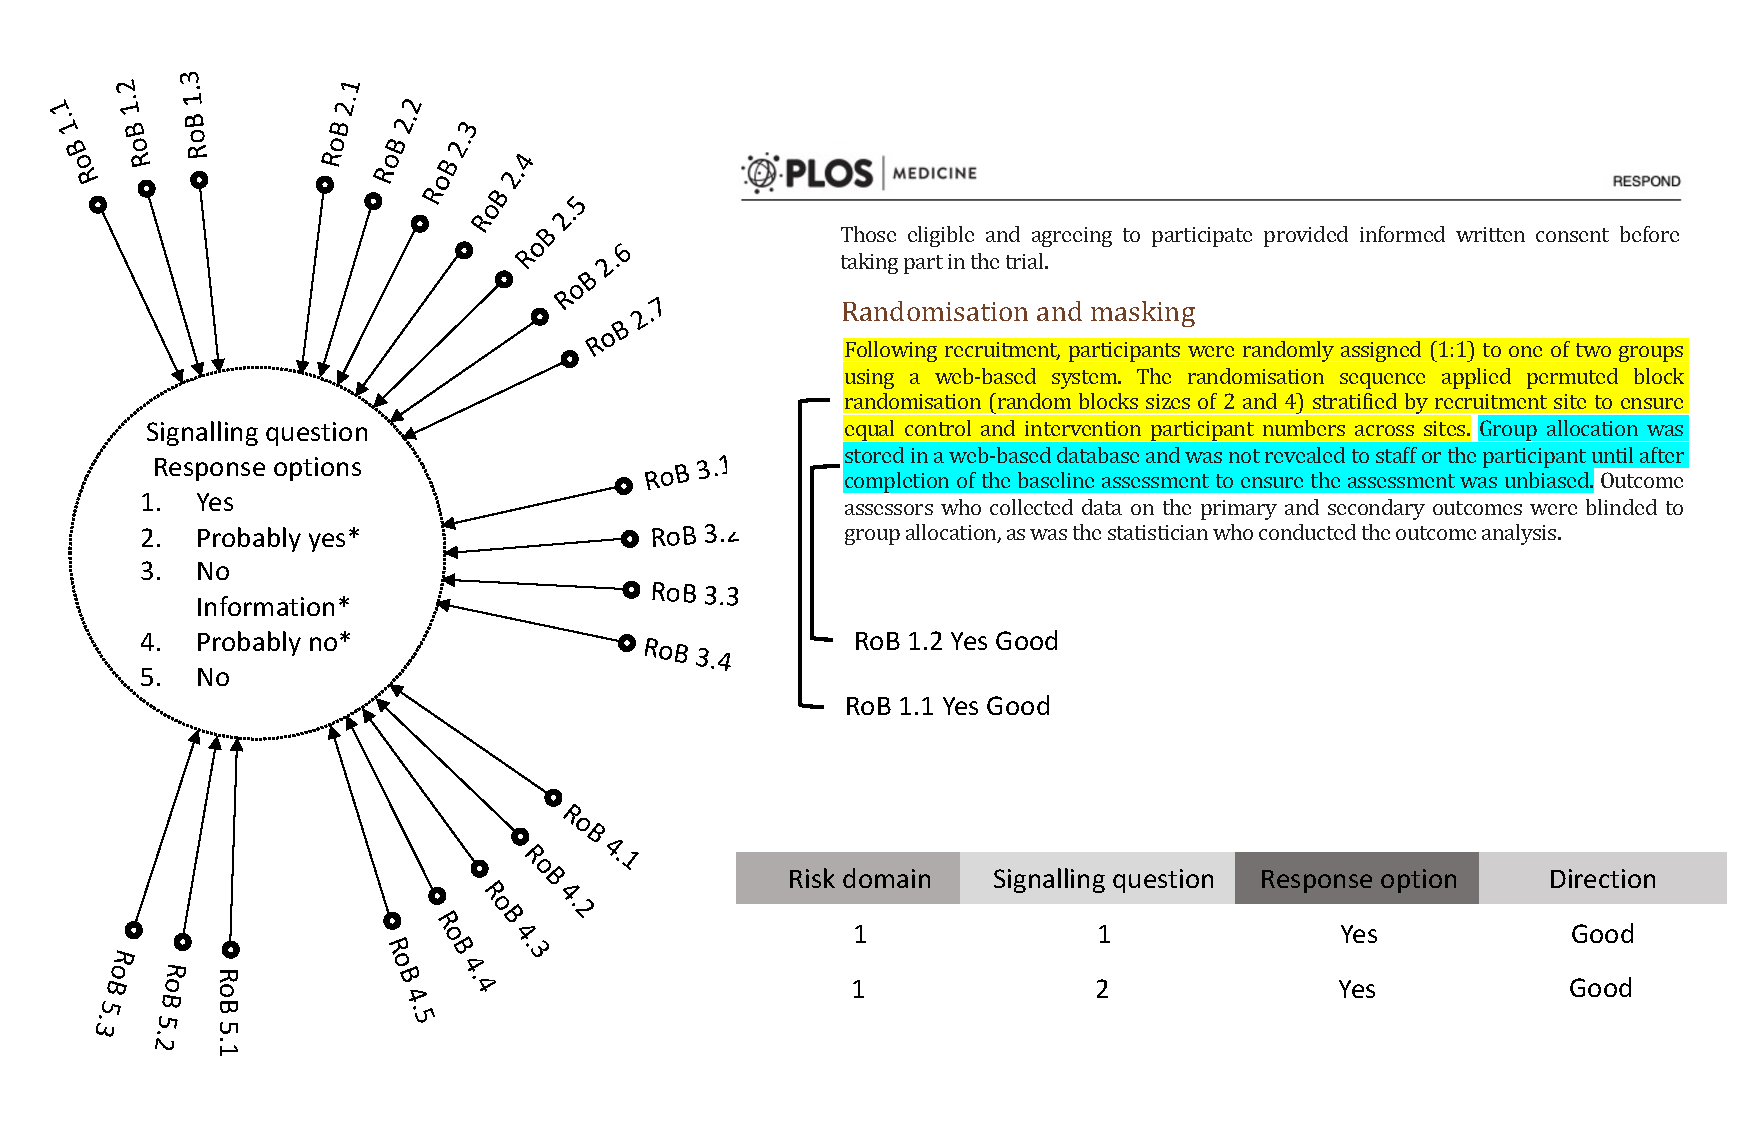
\includegraphics[width=0.90\columnwidth]{figures/annotation_schema.pdf}
    \caption{Our annotation scheme}
    \label{fig:annotationscheme}
\end{figure}
%
%
%



Creating a new annotated corpus involves defining an annotation scheme or adopting an existing one.
To our knowledge the only available annotation scheme for RoB span annotation was presented by ~\cite{dhrangadhariya2023first}.
Rather than creating a new scheme, we adapt and enhance their approach by learning from its drawbacks.
Their annotation scheme was directly adapted from the RoB 2.0 assessment procedure and hence it is imperative to understand the RoB 2.0 structure to understand the annotation scheme.
RoB 2.0 divides biases into five risk domains, each corresponding to different parts of the trial design.
Each risk domain decomposes into several signalling questions, each aiming to prompt a relevant response to bias assessment (refer to Table~\ref{tab1}).


%
%
%
\begin{table*}
 \centering
 %\captionsetup{justification=justified}
   \caption{The table lists down the bias domains as structured in the revised Cochrane RoB assessment tool (RoB 2.0) and the number of signalling questions (SQ) in each domain.}\label{tab1}
    \begin{tabular}{|l|l|r|}
    \hline
     Class & Domain & SQ\\
    \hline
    \hline
    RoB 1 & biases arising from the randomization process &  3\\
    RoB 2 & biases due to deviations from intended interventions & 7\\
    RoB 3 & bias due to missing outcome data & 4\\
    RoB 4 & bias in the measurement of the outcome & 5\\
    RoB 5 & bias in the selection of the reported result & 3\\
    \hline
    \end{tabular}
\end{table*}
%
%
%


The response options are restricted to ``Yes'', ``Probably yes'', ``No'', ``Probably no'', or ``No information''~\cite{sterne2019rob}.
Reviewers assess these signalling questions by examining the factual evidence in the RCT.
For instance, to answer the signalling question ``Was the allocation sequence random?'', the reviewer reads through the study to identify how participants were randomized into intervention groups.
If a well-executed method of randomization is identified, the reviewer answers with ``yes'' (the allocation sequence is random) judging the risk of bias for this signaling question as low risk.
Conversely, if a poorly executed method of randomization is found, the risk of bias is deemed  high risk with response option ``no''.
%Similarly, each signalling question prompts the reviewer to look for a piece(s) of factual evidence in the clinical study to respond with one of the five response options.



In RoB span annotation, we mimic this assessment process by considering evidence text spans in the RCT as the main units of annotation. 
Each span corresponds to answering a signalling question and is annotated with the most informative label. 
The label incorporates information about the signalling question number and the domain it assesses (for the above example, ``1.1'' for the first domain and first signalling question of the domain)
Additionally, the response judgement is incorporated in the label, such as ``1.1 Yes Good'' for a well-executed randomization (see Figure~\ref{fig:annotationscheme}).
Dhrangadhariya \textit{et al.} suggests collapsing the response options ``yes'' and ``probably yes'' into a single ``yes'', and ``no'' and ``probably no'' together into a single ``no'' to increase the inter-annotator agreement (IAA)~\cite{dhrangadhariya2023first}.
Except for some special case signalling questions, we too collapse these response option as suggested.
As shown in Figure~\ref{fig:flowchart} responding to any signalling question for the risk domain 2 as either ``Probably yes'' or ``Yes'' does not alter the final risk judgment for this domain (low, high, or some concerns).
In summary, the reviewer needs to label the identified text span with the RoB entity along with one of the response options.
In this regard, we have a hierarchical span annotation scheme comprising 22 entities corresponding to the 22 signalling questions, each with typically two response options and two directions (mutually exclusive).
We also remove the ``No Information'' labels since it is meant for the situations where actually no text evidence is found to answer a SQ leaving on text to be labelled with it.
However, for selected signalling questions, ``probably yes'', ``probably no'' and ``No Information'' may still be used.
For example, consider that an RCT uses ``...random number generator and sealed envelopes for patient randomization...'', but the trial provided no information on whether the envelop was ``opaque'' or not.
In such situations, ``No Information'' label is acceptable.
%Additionally, it is based on this span, the response judgment option is decided, and therefore even the response judgement information is incorporated in the label.
%Consider the following span is found to answer the above-mentioned signalling question, ``randomized participants using random number generation...'', which is a good randomization procedure and therefore the reviewer responds with ``yes''.
%The label extends the example label to ``1.1 Yes''.
%In addition, a direction is also added to the label, for example, whether it is ``good'' or ``bad.
%In this example, a good randomization ensure low risk for this signalling question and vice versa.
%Adding direction extends the example label to ``1.1 Yes Good''.


%
%
%
\begin{figure}
    \centering
    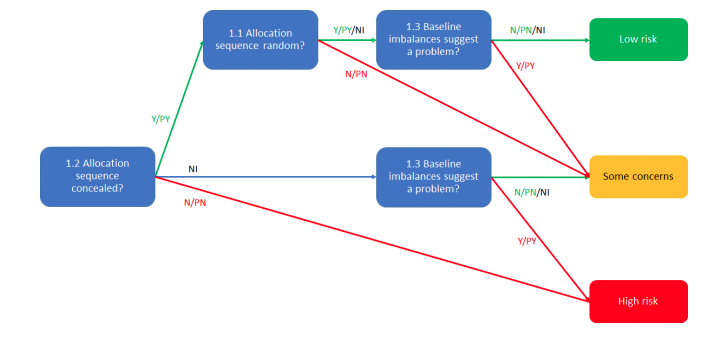
\includegraphics[width=0.60\columnwidth]{figures/rob1_flowchart.png}
    \caption{Algorithm for suggested judgement of risk of bias arising from the randomization process. Taken from the revised Cochrane's risk of bias tool (RoB 2.0).}
    \label{fig:flowchart}
\end{figure}
%
%
%


%
%
%
\subsection{Guideline development}
\label{guidelines}
%

Subjectivity in the revised Cochrane RoB 2.0 tool. %Anjani: Comments from Roger and Martin about the inherent subjectivity
%The signalling questions are broadly factual but leave room for subjective judgements and aim to facilitate judgements about the risk of bias.

The visual annotation placards were created based on the revised RoB 2.0 tool and were developed collaboratively by our team of experts.
Our team consisted of four researchers specializing in RoB assessment in physiotherapy and rehabilitation domains, including an epidemiology researcher, an assistant professor, a post-doc, and a PhD student.
Additionally, two researchers with expertise in natural language processing (NLP) were involved, one being a professor and the other a PhD student in computer science.
The inclusion of NLP researchers was particularly important because the guidelines and placards they helped create will be utilized to annotate a text corpus, which will serve as a benchmark for the NLP task of RoB span extraction.
Annotation guidelines along with the visual placards are detailed in the Supplementary material. %TODO: Prepare supplementary material
%
%
%
\subsection{Data collection}
\label{data}
%
The epidemiology researcher from our team created an annotation dataset of 60 RCTs from the domain of physiotherapy and rehabilitation.
Our corpus is focused on these domains because our annotators have RoB assessment expertise in this domain.
To ensure different outcome types are represented in the corpus, we restricted including XX, XX and X RCTs addressing subjective, objective and mortality primary outcomes.
In context of RCTs, subjective outcomes are measurements that rely on individuals' perceptions, opinions, or feelings about their own health or well-being.
These outcomes are typically self-reported by the participants in the trial.
Since they are based on individual experiences, they can be influenced by factors such as bias, expectations, or interpretation.
For example, pain intensity and quality of life.
Objective outcomes are measurements that are independent of individual opinions or perceptions and are based on observable and measurable data.
These outcomes are typically collected by trained assessors or through laboratory tests, imaging studies, or other objective methods.
For example, blood pressure, heart rate and other laboratory results.
Mortality outcomes refer to the occurrence of death during the course of the randomized controlled trial. 
These 60 studies were selected from four journals: journal 1, journal 2, journal 3 and journal 4. 
PDFs of the full-text RCTs were extracted and each article was collated with its trial protocol wherever available.
%TODO Anjani: Justify why only these journals were considered?
All these RCT PDFs have CC-BY-0 licences.
We list these studies and their licenses are listed in the supplementary material.
%TODO Anjani: Add if some studies were randomly added. Ask Roger for more information.


%\begin{itemize}
%    \item 60 RCTs
%    \item Between 2001:2021
%    \item CC0, CC BY, CC BY non-commercial
%    \item Eutils search - Include search query for PubMed
%    \item Search for each year, retmax=not defined, randomly selected 20 studies from the retrieved
%    \item Take the first three studies with free-full text available.
%    \item Upload to tagtog
%\end{itemize}
%
%
%
\subsection{Annotation}
\label{annotation}
%
Tagtog~\footnote{\url{https://www.tagtog.net/}}, a commercial text annotation web application, allows for annotating PDF (Portable Document Format) documents, was used for the annotation~\cite{cejuela2014tagtog}.
Out of the 60 documents, 9 were doubly annotated by two experienced annotators (a epidemiology researcher and an assistant professor) to calculate inter-annotator agreement (IAA) over these documents and the rest were singly annotated by the epidemiology researcher.
After the annotation of 9 doubly-annotated RCTs, we had to stop using tagtog for certain reasons and switched to the PAWLS annotation tool, which allows users to annotate PDFs for free~\cite{neumann2021pawls}.
We chose to annotate PDFs rather than plain text because RCT PDFs have a visual format (maintains the structure of sections and subsections, tables, and figures) that makes the annotation task quicker for the annotators and increases annotation quality.
Post annotation, the feedback was taken from both the annotators details of which could be found in the supplementary material. %TODO Anjani: Prepare the supplementary material 
%
%
%
\subsection{Conflict resolution}
\label{conflicts}
%
Conflict resolution and placard improvement.
Followed by annotating 49 more RCTs.
%
%
%
\subsection{Inter-Annotator Agreement}
\label{subsec:corpus}
%
Cohen's kappa is the standard annotation reliability measure for many classification annotation tasks, but it is not a relevant measure for token-level annotation tasks like the RoB annotation we carried out.
Therefore, we stick to reporting the pairwise F1 measure that disregards out-of-the-span tokens (unannotated tokens), which is the ideal measure of annotation reliability for the token-level annotation tasks~\cite{brandsen2020creating,deleger2012building}.
We interpret F1 measure as shown in the Table~\ref{tab:iaa_interpret}~\cite{landis1977measurement}.


%
%
%
\begin{center}
 \begin{table}[ht]
   \caption{The table details interpretation of pairwise F1-measure and Cohen's Kappa.}\label{tab:iaa_interpret}
 \centering
    \begin{tabular}{|l|r|}
    \hline
    Agreement interpretation & IAA range \\ 
    \hline
    \hline
        Poor & 0-0.99 \\ 
        Slight & 1 - 20.99 \\ 
        Fair & 21 - 40.99 \\ 
        Good & 41 - 60.99 \\ 
        Substantial & 61 - 80.99 \\ 
        Almost perfect & 81 - 99.99 \\ 
        Perfect & 100 \\ 
    \hline
    \end{tabular}
 \end{table}   
\end{center}
%
%
%
%
%
%
\subsection{LLM evaluation}
\label{llms}
%
We carry out the human evaluation of LLMs using detailed prompts in which LLMs are prompted to extract sentences from RCT PDFs that act as text evidence to answer a signalling question.
Basically the LLMs need to the same task as human annotators and they will be evaluated on the basis of correctness of the answer.
If the text selected by LLMs is a part of the human selected text, then we attribute it as a correct answer.
We use the publicly available ChatPDF tool for the purpose~\footnote{\url{https://www.chatpdf.com/}}.


% Why are we conducting an LLM evaluation and not classical machine learning?
Initially the annotation guidelines and annotations were adapted for classical machine learning and not large language models.
So even though we were annotating PDFs, we had to restrict a lot of annotations based on the assumption that PDF will be converted into text via OCR (optical character recognition) losing its structure of tables and figures, which anyway a classical machine learning model could not use without some modifications.
With the advent of LLMs and tools like ChatPDF which allows directly interactions of ChatGPT with PDFs, it was essential to evaluate these instead of forcefully adapting the task to a classical machine learning problem.
%
%
%
\section{Results}
\label{sec:results}
%
This section describes the results of the annotation project.

%
%
%
\begin{table}[!ht]
    \caption{IAA before after guidelines improvement}
    \label{table:IAA_sq}
    \centering
    \begin{tabular}{llll}
    \hline
        Signalling question & before guideline improvement & after guidelines improvement & change \\
    \hline
        RoB 1\_1 & 24.44 & 55.02 & +30.58 \\ 
        RoB 1\_2 & 50.28 & 44 & -6.28 \\ 
        RoB 1\_3 & 20.44 & 90.9 & +70.46 \\ 
        RoB 2\_1 & 1.34 & 67.26 & +65.92 \\ 
        RoB 2\_2 & 7.23 & 38.66 & +31.43 \\ 
        RoB 2\_3 & 5.42 & 0 & -5.42 \\ 
        RoB 2\_4 & - & 0 & 0 \\ 
        RoB 2\_5 & 0 & 0 & 0 \\ 
        RoB 2\_6 & 68.85 & 83.25 & +14.4 \\ 
        RoB 2\_7 & 6.52 & 0 & -6.52 \\ 
        RoB 3\_1 & 23.57 & 39.68 & +16.11 \\ 
        RoB 3\_2 & 0 & ~ & 0 \\ 
        RoB 3\_3 & 0 & 0 & 0 \\ 
        RoB 3\_4 & 0 & 0 & 0 \\ 
        RoB 4\_1 & 6.51 & 61.71 & +55.2 \\ 
        RoB 4\_2 & 0 & 0 & 0 \\ 
        RoB 4\_3 & 13.85 & 30.21 & +16.36 \\ 
        RoB 4\_4 & 0 & 56.25 & +56.25 \\ 
        RoB 4\_5 & 0 & 0 & 0 \\ 
        RoB 5\_1 & 0 & 0 & 0 \\ 
        RoB 5\_2 & 0 & 49.49 & +49.49 \\ 
        RoB 5\_3 & 0 & 0 & 0 \\ \hline
    \end{tabular}
\end{table}
%
%
%
\section{Discussion}
\label{sec:discussion}
%
After the first batch of documents (n=9) was annotated and the F1 measure IAA calculated, we saw some questions had zero agreement.
Our aim was to use the annotated corpus and resolve the conflicts between the annotators to increase the annotation agreement and also improve the instructions in the placards.
For multiple conflicting cases, the instructions were either unclear, interpreted differently, or the annotators forgot to annotate.
However, when the annotators went through the conflicts, they were able to resolve them.
Therefore, we recommend semi-automation for RoB information extraction given two succinct reasons.
Reason 1: Cognitive load of annotating (and assessment). Machine learning models can help function like ``hint finding'' for many questions.
Reason 2: Subjective judgments within the signalling questions.
%
%
%
\subsection{LLM evaluation}
\label{disc:llm}
%
We had a few examples where ChatPDF generated an answer to the signalling question, but these sentences comprising the answer were not to be found in the input PDF document.
After instructing ChatPDF to look into the uploaded PDF and not generate sentences by itself, it gives the following output.
``I apologize, but as an AI language model, I do not have access to any uploaded PDFs or any external sources. Please provide me with the PDF you are referring to, and I will be happy to extract the sentences related to answering the signalling question RoB 1.1.''
When no information was found to answer a RoB question, ChatPDF generates a response by itself giving example sentences that could be used to answer that question.
Can retrieve multiple related answers for a RoB question prompt and one of that has to be the correct answer and should be the same as what the annotators annotated.

%
%
%
\section{Conclusion}
\label{sec:conclusion}
%
XoX
%
%
%
\section{Abbreviations}%% if any
%
\begin{enumerate}
    \item RCT - Randomized Controlled Trial
    \item RoB - Risk of Bias
    \item SR - Systematic review
    \item LLM - Large Language Model
    \item GPT - Generative Pre-trained Transformer
    \item NLP - Natural Language Processing
\end{enumerate}
%
%
%
\backmatter

\bmhead{Supplementary information}

If your article has accompanying supplementary file/s please state so here. 

Authors reporting data from electrophoretic gels and blots should supply the full unprocessed scans for key as part of their Supplementary information. This may be requested by the editorial team/s if it is missing.

Please refer to Journal-level guidance for any specific requirements.

\bmhead{Acknowledgments}

%Acknowledgements are not compulsory. Where included, they should be brief. Grant or contribution numbers may be acknowledged.

%Please refer to Journal-level guidance for any specific requirements.
This research was supported by HES-SO, Valais-Wallis. 

%
%
%
\section*{Declarations}
%
\subsection*{Funding}
%
This research was supported by HES-SO, Valais-Wallis. 
%
%
%
\subsection*{Conflict of interest}
%
The authors declare that they have no competing interests.
%
%
%
\subsection*{Competing interest}
%
The authors declare that they have no competing interests.
%
%
%
\subsection*{Ethics approval}
%
Not applicable
%
%
%
\subsection*{Consent to participate}
%
OXO
%
%
%
\subsection*{Consent for publication}
%
OXO
%
%
%
\subsection*{Data availability}
%
Availability of data and materials
%
%
%
\subsection*{Code availability}
%
Code availability 
%
%
%
\subsection*{Authors' contributions}
%
Authors' contributions
BMC journals: \url{https://www.biomedcentral.com/getpublished/editorial-policies}
%
%
%
%%===================================================%%
%% For presentation purpose, we have included        %%
%% \bigskip command. please ignore this.             %%
%%===================================================%%
%
\begin{appendices}
%
%
%
\section{Annotation guidelines}\label{annot_guidelines}
%
An appendix contains supplementary information that is not an essential part of the text itself but which may be helpful in providing a more comprehensive understanding of the research problem or it is information that is too cumbersome to be included in the body of the paper.
%
%
%
\end{appendices}

%%===========================================================================================%%
%% If you are submitting to one of the Nature Portfolio journals, using the eJP submission   %%
%% system, please include the references within the manuscript file itself. You may do this  %%
%% by copying the reference list from your .bbl file, paste it into the main manuscript .tex %%
%% file, and delete the associated \verb+\bibliography+ commands.                            %%
%%===========================================================================================%%

\bibliography{bibliography.bib}% common bib file
%% if required, the content of .bbl file can be included here once bbl is generated
%%\input sn-article.bbl


\end{document}
